\documentclass[11pt, a4paper]{article}
\usepackage[ a4paper,left = 22mm, right=22mm,
	top=1.3cm, bottom=2cm,
	includehead, includefoot,
	headheight=3 cm]{geometry}
\usepackage[ngerman]{babel}
\usepackage[T1]{fontenc}
\usepackage[utf8]{inputenc}
\usepackage[dvips]{graphicx}
\usepackage{calc}
\usepackage{makeidx}
\usepackage{xcolor}
\usepackage{amsmath,amssymb}
\usepackage{subcaption}
\usepackage{hyperref}
\usepackage{multirow}
\usepackage{fancyhdr}
\usepackage{enumitem}
\usepackage{lastpage}
\usepackage{sectsty}
\usepackage{multirow}

\usepackage{titlesec}
\usepackage{enumitem}
\usepackage{titletoc}
\usepackage{amsmath}
\usepackage{pdfpages}
\usepackage{booktabs}
\usepackage{blindtext}


\usepackage[most]{tcolorbox}




\PackageWarningNoLine{multirow}{warning text}


\allsectionsfont{\sffamily}
\usepackage{eso-pic}
\newcommand\BackgroundWave{%
	\put(0,0){%
		\parbox[b][\paperheight]{\paperwidth}{\vfill \centering \vspace{12.0cm}
			
\includegraphics[width=\paperwidth]{logo/hsel-welle-grey}\vfill }}}%%
\begin{document}
\AddToShipoutPicture{\BackgroundWave}
\begin{titlepage}

\hspace{-1.0cm}
% \hspace{-2.0cm}
\begin{tabular}{p{8.0cm} p{8.0cm}}
  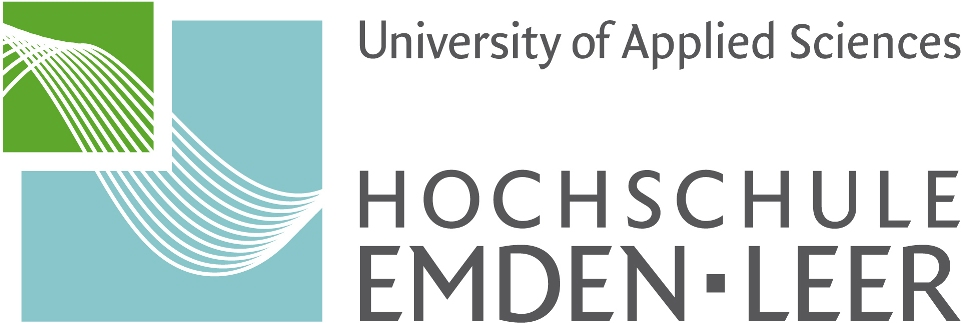
\includegraphics[width = 6.0cm]{img/Technik.png} &
   \parbox[b]{8.0cm}{
     {\large 	Fachbereich Technik }\\
     {\large 	Abteilung Elektrotechnik und Informatik }     
    } \\
   \\
   \hline
\end{tabular}
%
\begin{center}

\vspace{2.5cm}
\LARGE{\textsc{Formelsammlung Elektrotechnik}}\\

\vspace{2cm}%
\large
Oliver Schmidt\hspace{2cm} Matr. Nr. 7023462

\vspace{1cm} 
Emden, \today


\end{center}
\normalsize
\end{titlepage}

\newpage
\pagestyle{fancy}
\fancyhead[L]{{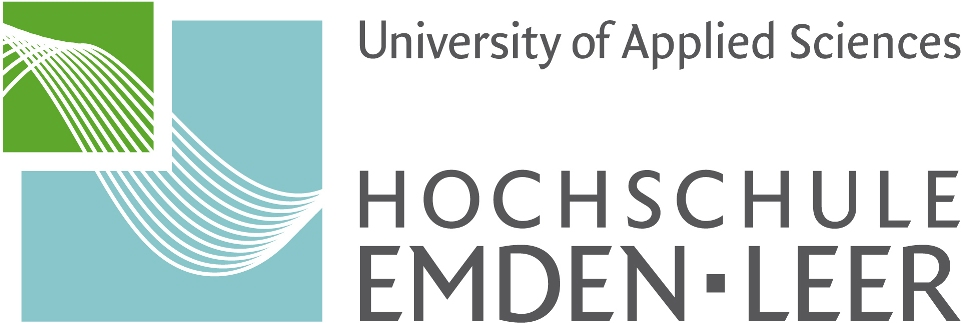
\includegraphics[width = 6.0cm]{img/Technik.png}}}
\fancyhead[R]{
	\Large{{
				Formelsammlung\\
				}}}
\fancyfoot[L]{\rightmark}
\fancyfoot[R]{Seite \thepage\ von \pageref{LastPage}}
\fancyfoot[C]{}
\renewcommand{\footrulewidth}{0.4pt}% Default \footrulewidth is 0pt

\pagenumbering{Roman}
\tableofcontents
\newpage
\listoffigures
\addcontentsline{toc}{section}{Abbildungsverzeichnis}
\newpage
\listoftables
\addcontentsline{toc}{section}{Tabellenverzeichnis}
\newpage
\ClearShipoutPicture

\pagenumbering{arabic}
\section{Elektrische Energietechnik}

\subsection{Thermische Kraftwerke}
\textbf{Wichtige Einheiten und Formelzeichen}:
\section{Reale Versuche}

\subsection{A Analog-Digital-Umsetzer (ADU)}



\end{document}
